\documentclass[conference]{IEEEtran}
\IEEEoverridecommandlockouts
% The preceding line is only needed to identify funding in the first footnote. If that is unneeded, please comment it out.
\usepackage{cite}
\usepackage{amsmath,amssymb,amsfonts}
\usepackage{algorithmic}
\usepackage{graphicx}
\usepackage{textcomp}
\usepackage{xcolor}
\usepackage{hyperref}
\usepackage{amsmath}
\usepackage{amssymb}

\newcommand{\rom}[1]{\uppercase\expandafter{\romannumeral #1\relax}}

\DeclareMathOperator*{\argmin}{arg\,min}

\def\BibTeX{{\rm B\kern-.05em{\sc i\kern-.025em b}\kern-.08em
    T\kern-.1667em\lower.7ex\hbox{E}\kern-.125emX}}
\begin{document}

\title{Assignment 5: a mathematical essay on random forest\\}


\author{\IEEEauthorblockN{Gautham Govind A}
\IEEEauthorblockA{\textit{Dept. of Electrical Engineering}\\
\textit{Indian Institute of Technology Madras} \\}
\textit{ee19b022@smail.iitm.ac.in}

}

\maketitle

\begin{abstract}
The objective of this assignment is to explore the mathematical formalism behind random forest classifier and then to use it in a real-life application. In this assignment, as a real-life application, random forest classifier is used to formally identify the factors which could have been used to predict how acceptable a car is from the popular car evaluation dataset. Data visualization, cleaning and modelling is done using Python. The analysis enables us to arrive at the conclusion that it is possible to make reasonable predictions regarding the acceptability of a car using factors including but not limited to safety rating, price and luggage boot space. 
\end{abstract}

\begin{IEEEkeywords}
random forest, python, visualization, predictive modelling, multinomial classification
\end{IEEEkeywords}

\section{Introduction}

Given a set of features and a target variable, predictive modelling is typically used for generating a model which can make predictions for cases where we do not know the value of the target variable, i.e., only the features are available. Apart from this use, a model can also be used for developing an intuition of how various factors influence the target variable. In this assignment, we try to make use of a model for the purpose of identifying the key factors which influence the decision in a classification problem.

In particular, we make use of random forest classifier for the purpose of identifying relationships in a classification problem. Random forests are among the most popular machine learning algorithms as they generate reasonable predictions across a wide range of data while requiring little configuration. Random forest is an ensemble learning method that operates by constructing a multitude of decision trees at training time. Random decision forests essentially correct for decision trees' habit of overfitting to their training set. It is a very flexible classifier in the sense that it can accommodate both continuous and categorical variables. In our particular problem, we will restrict ourselves to a classification problem using categorical variables.


In our problem setting, the goal is to use random forest classifier to predict the acceptability level of a car given a variety of factors like price, number of doors, passenger capacity, luggage boot space and safety rating. We make use of the publicly available car evaluation dataset for building the model. After building the model, we evaluate the model using a variety of evaluation metrics. By examining how well the model performs, we can identify how good the identified relationships are. Also, we check how critical each feature is to the prediction and create a ranking based on the importance of features.


Section \rom{2} gives an overview of the various techniques used for data cleaning, data visualization and an initial exploratory analysis. A lot of insights can be gained just by making qualitative observations from the given data. Section \rom{3} gives a short description of the mathematical formalism behind random forest. Section \rom{4} describes the various models that were tried and the results that were obtained by applying random forest in this particular case. Section \rom{5} gives a summary of the major conclusions drawn from the analysis.


\section{Exploratory Data Analysis}

In this section, we describe the process of data cleaning and data visualization. We also make some qualitative observations.

\subsection{Preliminary analysis}

The given dataset has 1728 rows and 7 columns. It must be noted that the dataset itself lacked any column headings: they had to be added in manually. A brief overview of the dataset is presented in Figure \ref{df_info}. We observe that we have \textbf{only categorical variables.} It also seems that there are no null values. 

We also look at the distribution for our target class, which is the acceptability rating termed 'target'. On plotting, we obtain Figure \ref{target_dist}. We have four categories: unacc (Unacceptable), acc (Acceptable), good (Good) and vgood (Very good). The count of cars in the unacceptable category is disproportionately high compared to other categories. We will have to account for this during model building.

\begin{figure}[tbh]
\centering
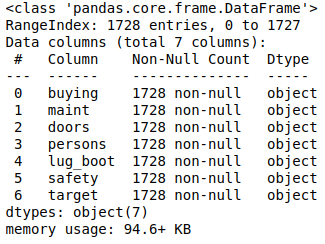
\includegraphics[scale = 0.50]{df_info.png}
\caption{Summary of the dataset}
\label{df_info}
\end{figure}

\begin{figure}[tbh]
\centering
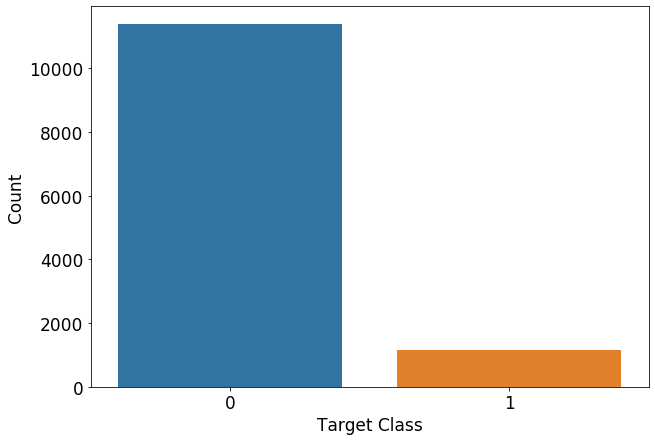
\includegraphics[scale = 0.39]{target_dist.png}
\caption{Target class imbalance}
\label{target_dist}
\end{figure}

\subsection{Feature by feature analysis}

Since all 6 features are categorical, for each feature we create a count plot, separating out the target classes. This can give qualitative insights regarding how a feature may affect the target variable. 

\subsection*{Buying price}

We obtain the count plot as shown in Figure \ref{bp}. We make the following observations:

\begin{itemize}
    \item Cars with high and very high buying price have a large proportion of unacceptable vehicles. Furthermore, there are no good or very good vehicles at this price range.
    \item Medium and low priced cars have representation from all four target categories.
\end{itemize}

Intuitively, this makes sense since people generally tend to find high prices unacceptable. For a deal to be considered good/ very good, it is almost always the case that the price should be on the lower end.

\begin{figure}[tbh]
\centering
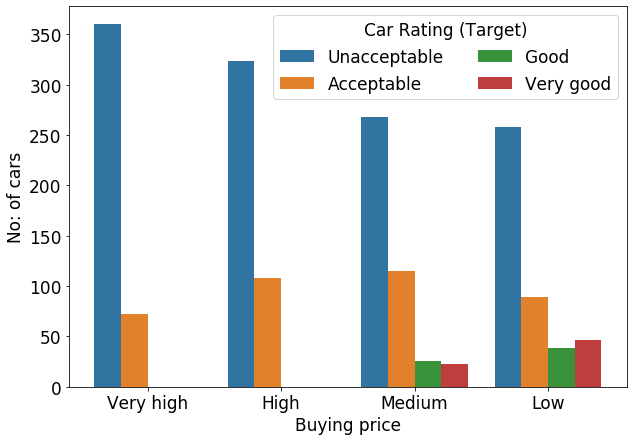
\includegraphics[scale = 0.39]{bp.png}
\caption{Distribution of buying price}
\label{bp}
\end{figure}

\subsection*{Maintenance price}

We obtain the count plot as shown in Figure \ref{mp}. We observe that the distribution is largely identical to the distribution for buying price. Again, we expect people to find high maintenance cost to be generally unacceptable.  

\begin{figure}[tbh]
\centering
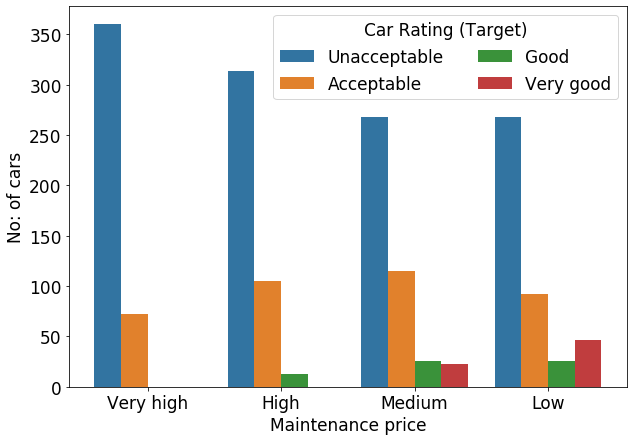
\includegraphics[scale = 0.39]{mp.png}
\caption{Distribution of maintenance price}
\label{mp}
\end{figure}

\subsection*{Number of doors}

We obtain the count plot as shown in Figure \ref{nd}. We observe that the distribution is largely identical for each category, i.e., irrespective of what the number of doors is, the distribution is same. In other words, the number of doors doesn't really provide any information regarding what would be the acceptability rating of a car. This implies that number of doors is not really a deciding factor as far as acceptance rating is concerned.

\begin{figure*}[tbh]
\centering
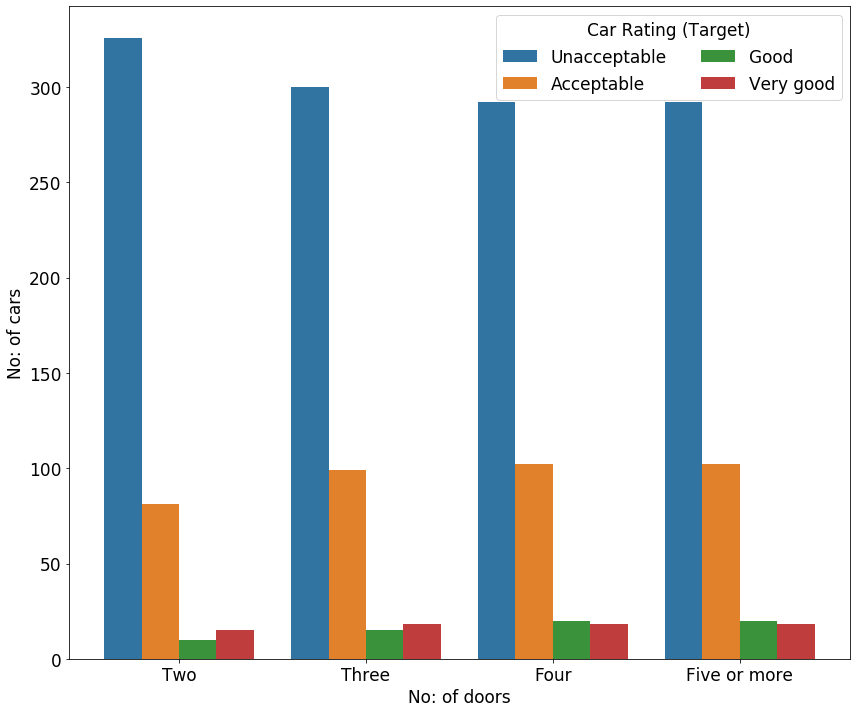
\includegraphics[scale = 0.4]{nd.png}
\caption{Distribution of number of doors}
\label{nd}
\end{figure*}

\subsection*{Passenger capacity}

We obtain the count plot as shown in Figure \ref{cp}. We make the following observations:

\begin{itemize}
    \item Cars that can accommodate only two people are all unacceptable.
    \item Cars which can accommodate four and more than four have similar distributions.
\end{itemize}

This seems to suggest that while having at least 4 seats is essential, beyond that the number of seats doesn't really have an impact on the acceptability rating.

\begin{figure}[tbh]
\centering
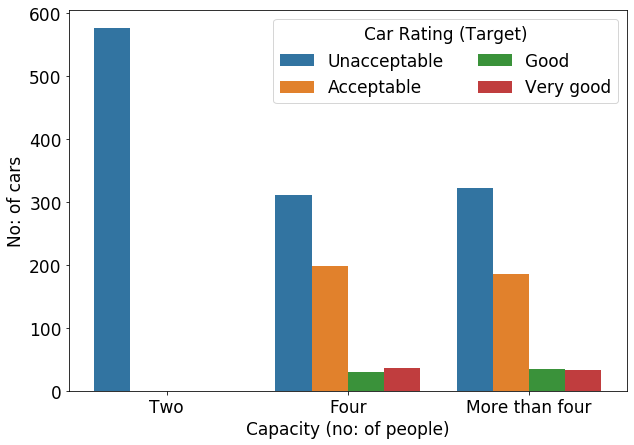
\includegraphics[scale = 0.39]{cp.png}
\caption{Distribution of passenger capacity}
\label{cp}
\end{figure}

\subsection*{Size of luggage boot}

We obtain the count plot as shown in Figure \ref{lgp}. We observe that though all categories have representation from all target categories, in general, the rating increases as the luggage boot size increases, which is what we would expect intuitively anyway.

\begin{figure}[tbh]
\centering
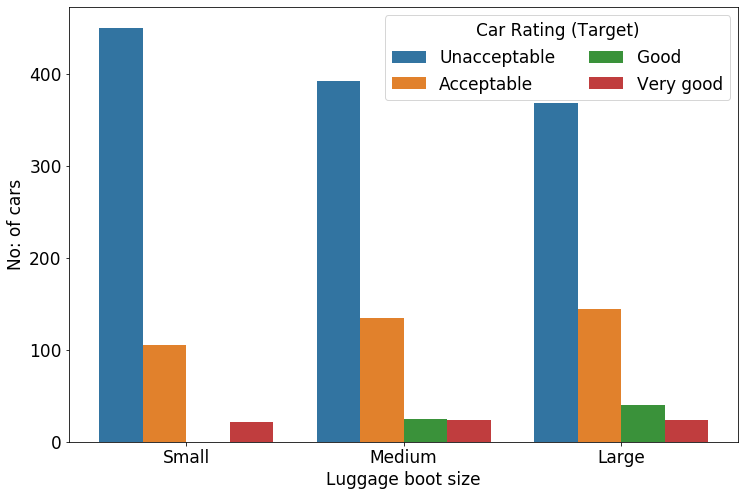
\includegraphics[scale = 0.33]{lgp.png}
\caption{Distribution of luggage boot size}
\label{lgp}
\end{figure}

\subsection*{Safety rating}

We obtain the count plot as shown in Figure \ref{sfp}. We make the following observations:

\begin{itemize}
    \item All low safety rated cars are unacceptable, which is what we would expect.
    \item As safety level increases, proportion of unacceptable cars decreases.
\end{itemize}

This seems to suggest that safety is a strong factor in predicting the acceptability of a car.

\begin{figure}[tbh]
\centering
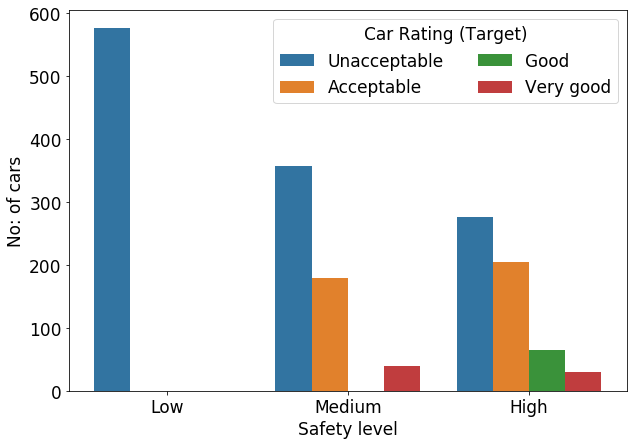
\includegraphics[scale = 0.39]{sfp.png}
\caption{Distribution of safety levels}
\label{sfp}
\end{figure}



\section{Model: Random Forest Classifier}

In this section, we will give a brief overview of the mathematical formalism behind the random forest classifier. 

Random forest is essentially an ensemble model made of a collection of decision trees. Decision trees have been discussed in great detail in the previous assignment. Ensemble methods use multiple learning algorithms to obtain better predictive performance than could be obtained from any of the constituent learning algorithms alone. 

The primary concern with decision trees is that they tend to overfit the data when suitable regularization techniques are not employed; random forest tries to overcome this problem. The idea behind random forest is simple: rather than relying on the prediction of a single tree, which can be inaccurate due to overfitting, train a large number of trees and make a decision using the predictions of all the trees. In the case of regression, this could be by making use of averaging, whereas in the case of classification this could be by taking the most voted class.

In other words, decision trees are essentially low bias, high variance classifiers. By averaging the predictions of several trees, we are bringing down the variance by incurring a marginal increase in bias. Therefore, random forests are low variance classifiers.  

To make things more concrete, we consider one case where random forests easily outperform decision trees. Consider the decision boundary shown in Figure \ref{dtvsrf_og}. Figure \ref{dtvsrf_q1} represents the decision boundary learnt by a decision tree. Since a decision tree can only have boundary segments parallel to either x-axis or y-axis, we end up with the boundary as shown in the this figure. However, since random forests average over a number of decision trees, it comes up with the decision boundary as shown in Figure \ref{dtvsrf_q2}. Clearly, this more closely resembles the decision boundary which we would like to learn.

\begin{figure}[tbh]
\centering

\includegraphics[scale = 0.35]{dtvsrf_og.png}
\caption{Decision boundary to be learned}
\label{dtvsrf_og}
\end{figure}

\begin{figure}[tbh]
\centering

\includegraphics[scale = 0.35]{dtvsrf_q1.png}
\caption{(Decision boundary learned by decision tree }
\label{dtvsrf_q1}
\end{figure}

\begin{figure}[tbh]
\centering
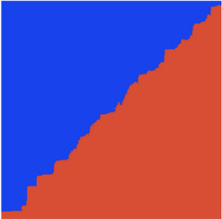
\includegraphics[scale = 0.35]{dtvsrf_q2.png}
\caption{Decision boundary learned by random forest}
\label{dtvsrf_q2}
\end{figure}

The major benefits offered by a random forest classifier are:

\begin{itemize}
    \item \textbf{Robust model:} The greatest advantage of a random forest model is that it is very robust. This means that it achieves very good performance on a variety of datasets with very minimal tuning. In many cases, random forest models can be used out-of-the-box, with very minimal hyperparameter tuning. 
    \item \textbf{Non-parametric approach}: Makes no assumptions of the training data or prediction residuals; e.g., no distributional, independence, or constant variance assumptions.
    \item \textbf{Requires little data preparation}: Other techniques often require data normalization. Since trees can handle qualitative predictors, there is no need to create dummy variables
\end{itemize}

Some limitations of this approach:
\begin{itemize}
    \item \textbf{Black-box model}: Although moving to a random forest from decision tree greatly improves model performance, this is achieved by sacrificing interpretability. Unlike decision trees, which are considered white-box models, random forests are black-box models in the sense that their results may not be easily explainable.  
    \item \textbf{Non-optimality}: Random forest learning algorithms are based on heuristics such as the greedy algorithm where locally optimal decisions are made at each node. This is because since random forests involve a large number of individual decision trees, it is not possible to train each tree optimally as this is computationally infeasible. The downside of heuristic algorithms is that they cannot guarantee globally solutions.
\end{itemize}





\subsection{Mathematical formalism}

A random forest is essentially an ensemble of decision trees. The output of a random forest can hence be thought of as some aggregation of the output of individual trees. Therefore, the mathematical principles underlying random forests are same as that of decision trees. A brief review of the mathematical formalism behind decision tree is given below.

What a decision tree essentially learns is a decision for each decision node. In particular, suppose a decision tree makes use of an impurity measure S (various measures for quality are discussed later). Suppose a node splits the dataset into two subsets left and right. Then the node computes the quantity:
$$ J(k, t_k) = \frac{m_\textrm{left}}{m}G_\textrm{left} + \frac{m_\textrm{right}}{m}G_\textrm{right} $$ where $m_\textrm{left}$ is the number of samples in the left subset, $m_\textrm{right}$ is the number of samples in the right subset, $S_\textrm{left}$ is the impurity measure for the left subset and $S_\textrm{right}$ is the impurity measure for the right subset. The attempt is to find the split which minimizes $J(k, t_k)$.

We can regard $J(k, t_k)$ as the cost function. The algorithm first splits the training set into 2 subsets using a single feature $k$ and a threshold $t_k$ . A pair $(t_k , k)$ is searched that minimizes the cost function the best. This procedure is repeated, looking for the best predictor and the best cut-point in order to split the data further so as to minimise the cost function. This process
continues till the set stopping criterion is reached or when every training sample is perfectly classified.

The above algorithm is repeated for a number of trees. The ensemble of trees are then used for making a prediction. Based on whether we sample the features themselves for each tree or not, we have two approaches: bagging and random forests. These will be examined in more detail in a later section.

An overview of two common attribute selection measures/ impurity measures is given below:

\begin{enumerate}

    \item Gini Index/Impurity: This is essentially a measure of total variance across the K classes.
    $$ G = \sum_{k=1}^{K}\hat{p_{i, k}}(1 - \hat{p_{i, k}}) $$ where $p_{i,k}$ is the ratio of class k instances among the training instances in the ${i^\textrm{th}}$ node. The Gini index takes on a small value if all of the $\hat{p}_{i,k}$ ’s are close to zero or one. So, small value implies that a node predominantly contains one class. And a zero value implies that the node is pure. Thus Gini index could also be viewed as a measure of impurity. The equation for Gini index can also be rewritten as:
    $$ G = 1 - \sum_{k=1}^{K}\hat{p_{i, k}^2} $$
    
    \item Entropy: The formulation has a close resemblance with the entropy formulation in thermodynamics. 
    $$ D = -\sum_{k = 1}^{K}\hat{p_{i, k}}\log{\hat{p_{i, k}}} $$ where again K is the total number of classes and $p_{i,k}$ is the ratio of class k instances among the training instances in the ${i^\textrm{th}}$ node. As was the case with Gini index, a smaller value of entropy signifies higher purity and a larger value of entropy signifies impurity.
\end{enumerate}



\subsection{Ensemble methods}

As discussed above, there are two approaches to creating an ensemble of decision trees: bagging and random forests. These are described below:

\subsubsection{Bagging}

Decision trees suffer from high variance and can be very non-robust, in general. This means that even a slight change or using a different set of samples from the dataset could lead to different trees. Bootstrap aggregation or Bagging is a procedure specifically useful for high capacity classifiers for reducing their variance. Bootstrapping is a technique to obtain data-points. We generally do not have access to multiple training sets and hence we do bootstrapping, i.e. we take repeated samples from the same training data set. Hence, we can sort of obtain a proxy for distinct datasets by repeatedly re-sampling observations from the original dataset. This sampling is done with replacement, meaning the same observation can occur in more than one of such synthetically generated datasets.

To apply bagging to trees, we simply construct B trees $f^1 (x), f^2 (x), .., f ^ B (x)$ using B bootstrapped training sets and average the resulting predictions to obtain a single low
variance statistical model. The constructed trees can be allowed to grow deep even if this means that they suffer from high variance, since averaging reduces variance and hence gives a better model. For classification, instead of averaging we take the most frequent prediction. Rest of the approach remains the same. B here would be a hyperparameter. High values of B just implies we are
averaging over many trees and hence apart from computational complexity, increasing B doesn't lead to overfitting. In practice, B is kept sufficiently large so that the error settles down.

\subsubsection{Random Forest}

Similar to bagging, we build a number of decision trees on bootstrapped training samples. But when building these decision trees, when each time a split is considered, a random
sample of $m$ predictors is chosen as split candidates from the full set of $p$ predictors.This also ensures a single feature is not influencing majority of decisions in all trees. Usually $m \approx \sqrt{p}$ but $m$ is in fact a hyper-parameter that could be chosen via cross validation. 

The main motivation behind random forest is the fact that prediction from individual trees of a bagged model tend to be correlated. Random forests help decorrelate the trees by making use of random sampling of features. The variance after averaging reduces in a much better fashion if the predictions from each tree are uncorrelated. The main advantage of bagging/random forest is that all the trees can
be trained in parallel and hence could be sped up easily by making use of some form of parallel training. But this kind of approach cannot be readily employed in sequentially/adaptively trained models, i.e. boosting based approaches.

\subsection{Time complexity}

In a decision tree, a split has to be found until a maximum depth $d$ has been reached. In the worst case, maximum depth is equal to n, the training set size. The strategy for finding a split is to look for a suitable threshold for each feature of the dataset. Since there are $p$ such variables, we make $np$ decisions per node. Considering a random forest with $n_\textrm{trees}$ such trees:
\begin{itemize}
    \item Assuming no-feature selection, the upper bound for train time complexity is $O(n_\textrm{trees} n^2 p)$.
    \item  If $\sqrt{p}$ random feature selection is done at each node, the upper bound for train time complexity is $O(n_\textrm{trees} n^2 \sqrt{p})$.
\end{itemize}




\section{Modelling }

In this section, we discuss the application of the random forest classifier to our problem. 

We create and evaluate two models:

\begin{enumerate}
    \item In Model 1, we do not do random sampling of features, i.e., we perform bagging.
    \item In Model 2, we perform random sampling of features.
\end{enumerate}

For each model, we take care to account for the inherent imbalance in the training dataset with respect to the target class. This is done by making use of appropriate weights during the training of each decision tree of the ensemble model.

We evaluate the models based on multiple metrics. A short description of the metrics used is given below:

\begin{itemize}
    \item \textbf{Accuracy:}
    Accuracy is simply the \textbf{ratio of number of correct predictions to total number of predictions.} Although this seems like a very good metric intuitively, accuracy fails on classification problems with a skewed class distribution because of the intuitions developed by practitioners on datasets with an equal class distribution.
    \item \textbf{Precision:}
    Precision is the \textbf{ratio of true positives to the total positive predictions.} Precision is typically used when the cost of false positive is high. For instance, email spam detection.
    \item \textbf{Recall:}
    Precision is the \textbf{ratio of true positives to the total positive ground truths.} Recall is typically used when the cost of false negative is high. For instance, in fraud detection or sick patient detection.
    \item \textbf{F1-score:}
    F1-score is simply a \textbf{harmonic average of precision and recall.} F1 Score is typically used if we need to seek a balance between Precision and Recall and there is an uneven class distribution.
    
    
\end{itemize}

It must be noted that, strictly speaking, precision, recall and f1-score are defined only for binary classification. However,for multi-class classification, we can define these metrics for each class separately. Furthermore, we can take averages of these measures across all classes to compute a global metric. This can be done through the following two metrics:
\begin{itemize}
    \item \textbf{Macro averaging:} In this method, a simple average is done without taking into account any class imbalance.
    \item \textbf{Weighted averaging:} In this method, averaging is done in a weighted manner after accounting for class imbalance using support, which is simply the number of instances belonging to a particular class according to true labels.
\end{itemize}

We will be using \textbf{weighted averaged f1-score} as the metric for comparison between models. The dataset is split into training, validation and test sets. The test set is kept aside and will be used only after choosing the best model. Comparison between models is done using validation set.

\subsection{Model 1}

In this model, we create a bagging model. The number of trees to be included is a hyperparameter. Essentially, we keep increasing the number of trees till the metric (weighted f1-score in our case) stabilizes. The plot of score against number of trees is shown in Figure \ref{bag_num}. Clearly, \textbf{the score stabilizes for a tree count of more than 400.} Hence, we set the number of trees equal to 400. Also note that we perform bootstrapping to create training sets for each individual tree. Two-thirds of the total number of datapoints is used for training each tree. The performance of the model on validation set is shown in Figure \ref{bag_info}. The table reports macro averages and weighted averages. The weighted averaged f1-score is \textbf{0.959.}

\begin{figure}[tbh]
\centering
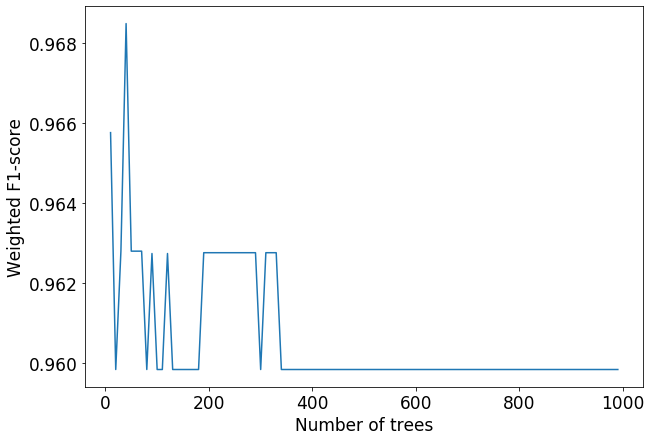
\includegraphics[scale = 0.34]{bag_num.png}
\caption{Evolution of f1-score with number of trees}
\label{bag_num}
\end{figure}

\begin{figure}[tbh]
\centering
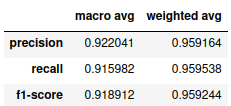
\includegraphics[scale = 0.75]{bag_info.png}
\caption{Metrics for model 1 }
\label{bag_info}
\end{figure}



\subsection{Model 2}

In this model, we create a random forest model, with feature sampling. The number of trees is set to be 400 (from the above analysis). In this case, the maximum number of features to be included while random sampling is taken as the hyperparameter. In our case, the total number of available features is only 6. Hence, we can perform a simple grid search from 1 through 6 for the number of features to be used while random sampling. The plot of score against number of features is shown in Figure \ref{rf_num}. Clearly, \textbf{the score achieves a peak for the number of features equal to 2.} Hence, we set the number of features during sampling equal to 2. Also note that we perform bootstrapping to create training sets for each individual tree. Two-thirds of the total number of datapoints is used for training each tree. The performance of the model on validation set is shown in Figure \ref{rf_info}. The table reports macro averages and weighted averages. The weighted averaged f1-score is \textbf{0.968. Clearly the model outperforms Model 1.}

\begin{figure}[tbh]
\centering
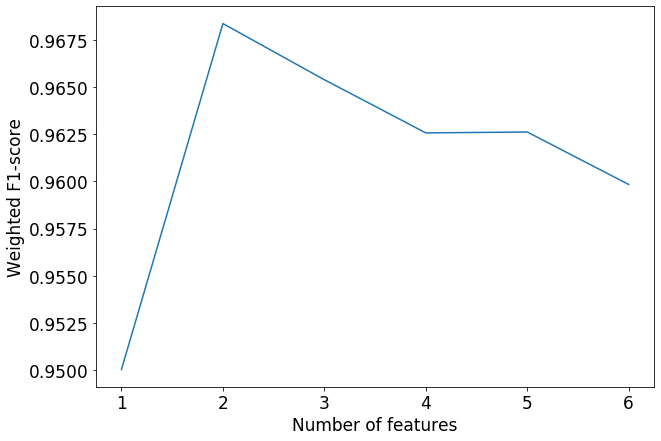
\includegraphics[scale = 0.34]{rf_num.png}
\caption{Evolution of f1-score with number of features}
\label{rf_num}
\end{figure}

\begin{figure}[tbh]
\centering
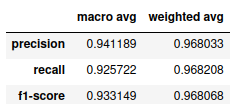
\includegraphics[scale = 0.75]{rf_info.png}
\caption{Metrics for model 2 }
\label{rf_info}
\end{figure}


\subsection{Best Model}

From the above analysis, we conclude that Model 2 performs the best. Hence, we train a random forest model with a random sampling of 2 features and 400 trees on the whole dataset consisting of training set and the validation set. We then evaluate this on the test set. The metrics for this final model is given in Figure \ref{met_best} and the confusion matrix is given in Figure \ref{cf_matrix}. 

To get a sense of the importance of features, we also calculate the feature importance scores of each feature using an in-built method provided by scikit-learn. Essentially, the importance of a feature is computed as the (normalized) total reduction of the criterion brought by that feature. It is also known as the Gini importance. A plot showing the feature importance scores is given in Figure \ref{feature_imp}. \textbf{It can be seen that safety rating is the most important feature, whereas number of doors is the least important feature.} It is noteworthy that this agrees with our analysis during the exploratory phase.

\begin{figure}[tbh]
\centering
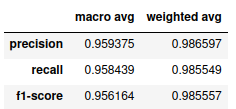
\includegraphics[scale = 0.75]{met_best.png}
\caption{Metrics for the best model }
\label{met_best}
\end{figure}

\begin{figure}[tbh]
\centering
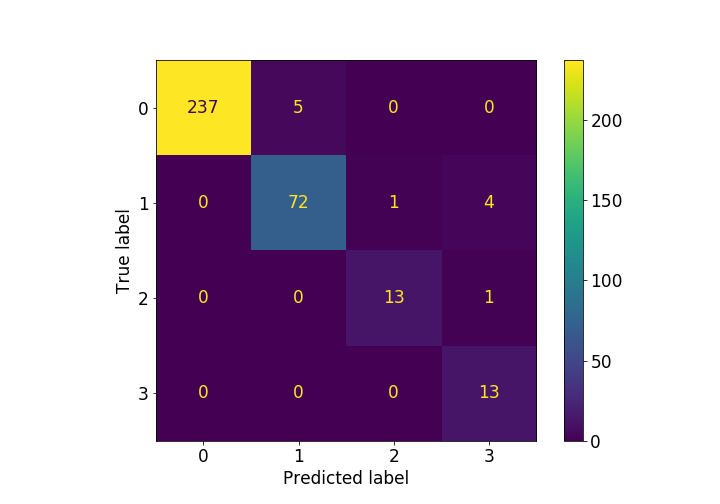
\includegraphics[scale = 0.34]{cfmatrix.png}
\caption{Confusion matrix for the best model}
\label{cf_matrix}
\end{figure}

\begin{figure}[tbh]
\centering
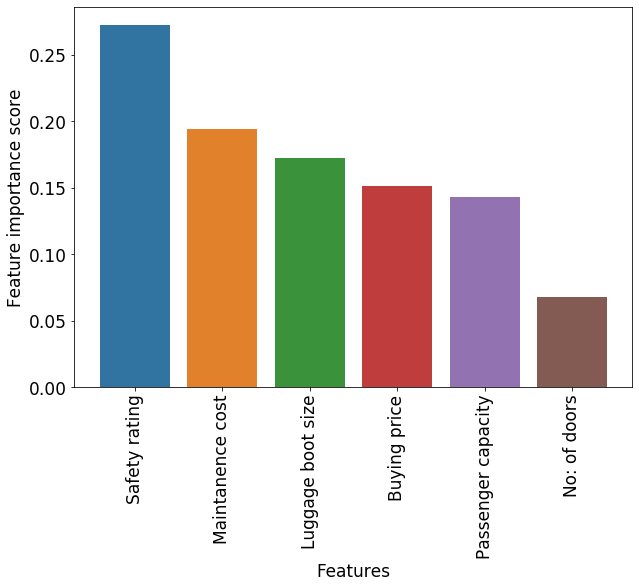
\includegraphics[scale = 0.34]{feature_imp.png}
\caption{Feature importance scores}
\label{feature_imp}
\end{figure}


\section{Conclusions}

From our extensive analysis of the given dataset using random forest classifier, we arrive at the following conclusions:

\begin{itemize}
    \item Random forest classifier performs very well on the given dataset. In fact, it performs better than the decision tree classifier which we created in the previous assignment. 
    \item Although random forest model performs better than the decision tree model, this improvement comes at the cost of reduced interpretability.
    \item Accuracy may not be a good measure of performance for imbalanced classification tasks. It is necessary to use metrics like weighted f1-score for such cases.
    \item Best performance is obtained by setting the number of randomly selected features to 2 and number of trees to 400.
    \item Safety rating is found to be the most important feature whereas number of doors is found to be the least important feature, as was also observed during the initial qualitative analysis.
\end{itemize}



\section{Avenues for further research}

Random forest classifier performs quite well for the given dataset. Doing some kind of feature preprocessing like PCA, to extract important features before inputting it to the model might help. Trying out boosting methods might also help improve the performance of the model.  



\nocite{*} % Print all references regardless of whether they were cited in the poster or not
\bibliographystyle{ieeetr}
\bibliography{sample} % Use the example bibliography file sample.bib


\end{document}

